\chapter{Detector}

\section{The Large Hadron Collider (LHC)}
Although the Standard Model of particle physics has been remarkably successful up to TeV scale, several fundamental questions remain unanswered. The Large Hadron Collider (LHC) at CERN is the most powerful particle accelerator ever built, designed to explore above the TeV energy scale. It consists of a 27-kilometer ring of superconducting magnets and accelerating structures, enabling proton-proton collisions at an unprecedented energy of 13 TeV (design energy of 14 TeV). The main purpose of the LHC is to explore the electroweak symmetry breaking for which the Higgs mechanism is presumed to be responsible and search for new physics beyond the Standard Model.
\begin{figure}[ht]
    \centering
    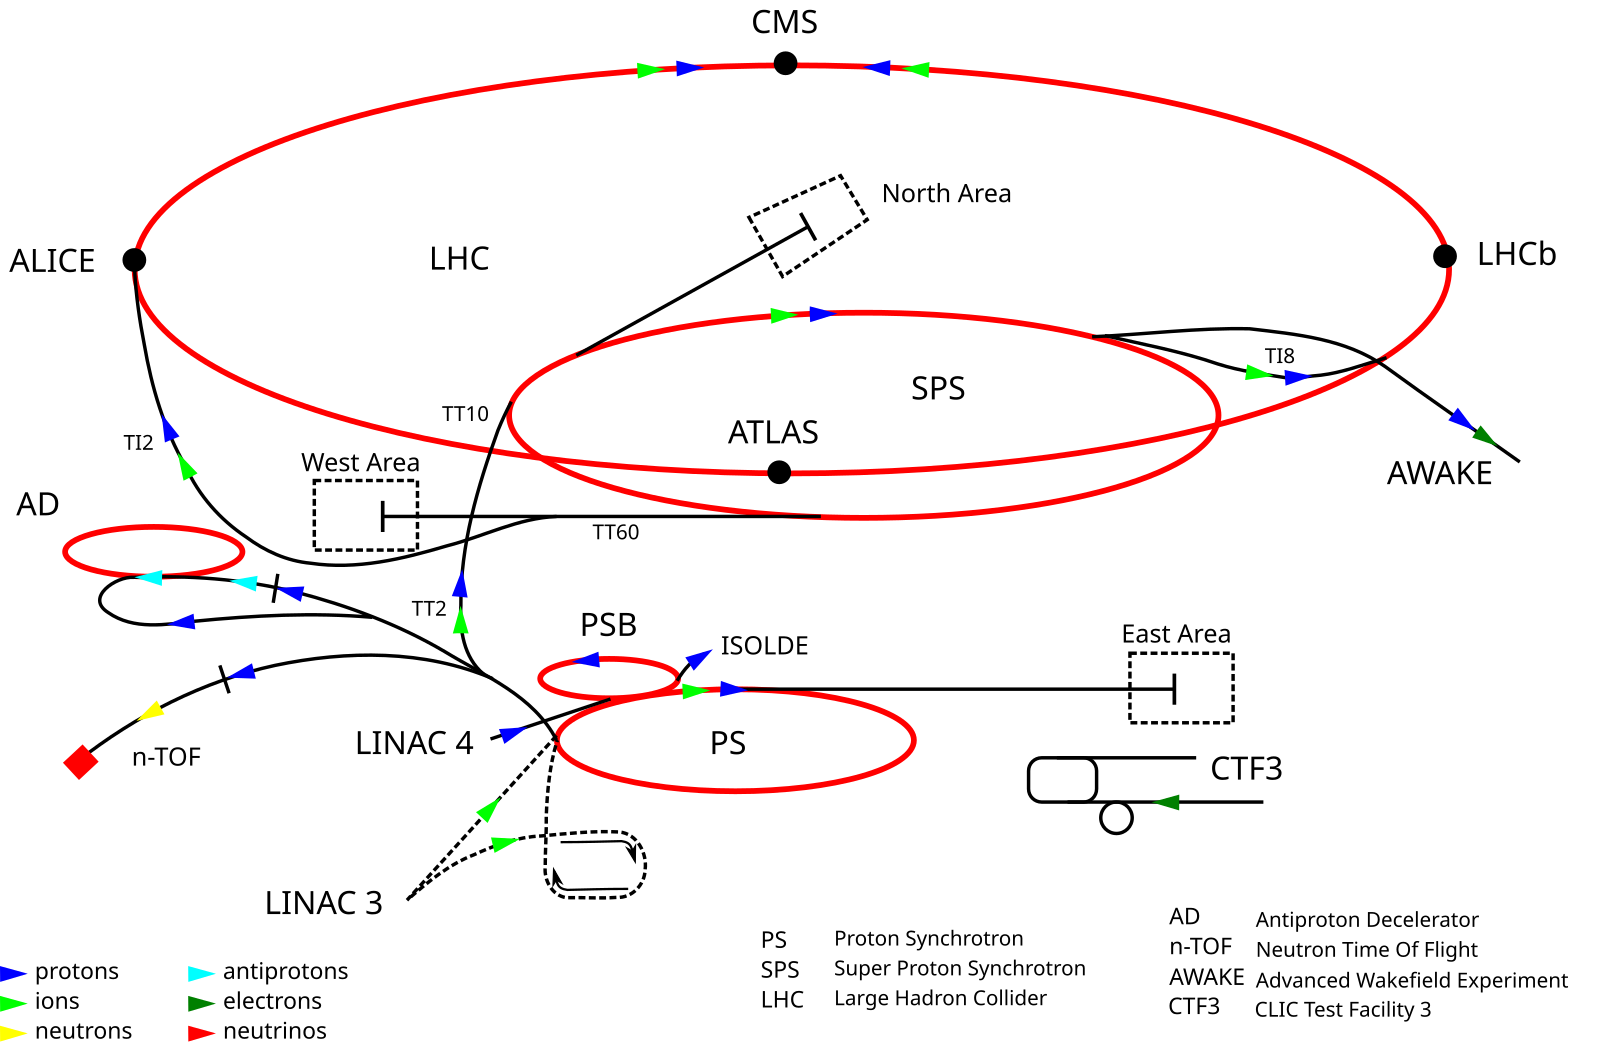
\includegraphics[width=0.8\textwidth]{Figures/Cern_Accelerator_Complex.png} % Replace with your LHC diagram file
    \caption{The schema of LHC} ~\cite{lhc_picture}
    \label{fig:lhc}
\end{figure}

The LHC features a high collision rate with 25 ns bunch spacing, producing up to $10^9$ interactions per second. The facility includes key experimental sites like CMS, ATLAS, LHCb, and ALICE, each optimized for specific research goals. The injection system consists of the Proton Synchrotron (PS) and Super Proton Synchrotron (SPS), ensuring high beam luminosity and energy.

\subsection{Key Components of the LHC}

\subsubsection{Injector Chain}
The LHC relies on a sequence of pre-accelerators to prepare the particle beams:
\begin{itemize}
    \item \textbf{Linear Accelerator (Linac4):} Replaced Linac2 and accelerates negative hydrogen ions (H$^-$) to 160 MeV. Synchrotron Booster (PSB). \cite{linac4}
    \item \textbf{Proton Synchrotron Booster (PSB):} Strips electrons from H$^-$ ions to produce protons and accelerates them to 2 GeV. \cite{psb}
    \item \textbf{Proton Synchrotron (PS):} Further increases the beam energy to 26 GeV.\cite{ps}
    \item \textbf{Super Proton Synchrotron (SPS):} Boosts the energy of protons to 450 GeV before injection into the LHC.\cite{sps}
\end{itemize}
Each stage ensures the beam achieves the required energy, intensity, and quality, culminating in proton-proton collisions at 13.6 TeV in the LHC in Run3.

\subsubsection{Main Ring}
The LHC ring consists of two counter-rotating beam pipes, maintained under ultrahigh vacuum conditions to avoid particle collisions with residual gas.
\begin{itemize}
    \item \textbf{Superconducting Magnets:} Approximately 1,232 dipole magnets steer the beams around the circular path, while quadrupole magnets focus them to maintain stability. \cite{superconducting}
    \item \textbf{Cryogenics:} The superconducting magnets operate at 1.9 Kelvin (-271\degree C), achieved using liquid helium cooling systems. \cite{lhc_2024}
\end{itemize}

\subsubsection{Experimental Sites}
The LHC includes four main experiments, strategically placed along the ring:
\begin{itemize}
    \item \textbf{CMS (Compact Muon Solenoid):} Focused on studying high-energy collisions for precision measurements and new physics.
    \item \textbf{ATLAS (A Toroidal LHC Apparatus):} Another general-purpose detector designed for broad physics exploration.
    \item \textbf{ALICE (A Large Ion Collider Experiment):} Specializes in studying heavy-ion collisions and the quark-gluon plasma.
    \item \textbf{LHCb (LHC Beauty Experiment):} Dedicated to investigating the matter-antimatter asymmetry by studying b-hadron decays.
\end{itemize}

\subsubsection{Collimation and Beam Dumps}
The LHC is equipped with a sophisticated collimation system to remove stray particles and protect sensitive components. Beam dumps allow controlled termination of particle beams after experiments or emergencies.

\subsubsection{Collision Points}
Particles are brought to collision points within the detectors, achieving a luminosity of $10^{34}~\mathrm{cm^{-2}s^{-1}}$. These conditions facilitate rare particle processes, such as Higgs boson production.

\subsection{Technological Challenges}
\begin{itemize}
    \item \textbf{Radiation Damage:} Extensive shielding is required to protect equipment and personnel from high levels of radiation.
    \item \textbf{Alignment Precision:} The alignment of the LHC's components must be maintained within micrometers to ensure proper beam steering.
    \item \textbf{Data Volume:} Experiments generate petabytes of data annually, necessitating advanced computational infrastructure for storage and analysis.
\end{itemize}

The LHC represents a pinnacle of human engineering and scientific collaboration, involving thousands of scientists and engineers worldwide.

\section{The Compact Muon Solenoid (CMS)}
CMS is a general-purpose detector optimized for high-precision measurements and searches for rare physics events. The detector design focuses on:
\begin{itemize}
    \item Precise tracking for charged particles.
    \item High-resolution electromagnetic and hadronic calorimetry.
    \item Efficient muon identification and momentum resolution.
    \item Robust missing transverse energy measurement.
\end{itemize}

\begin{figure}[ht]
    \centering
    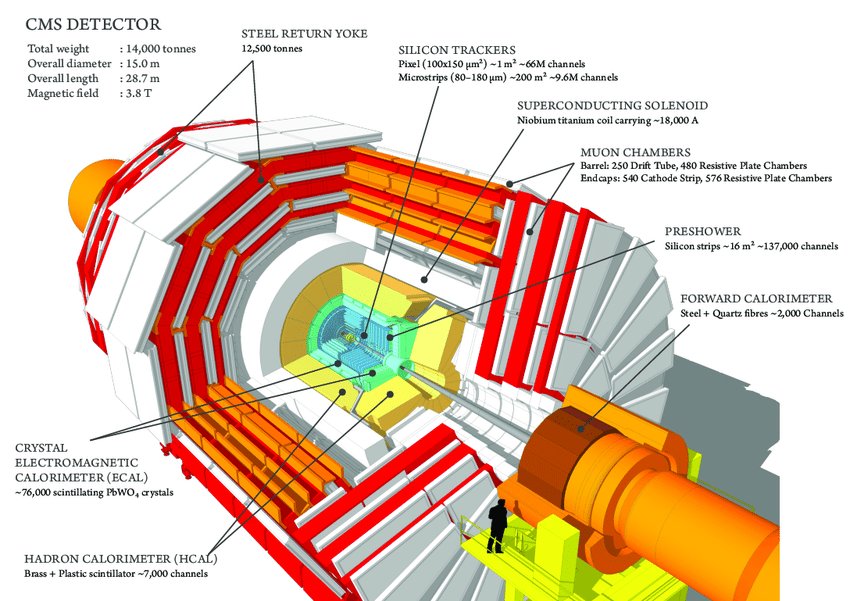
\includegraphics[width=0.8\textwidth]{Figures/CMS Detector Schematic.png} % Replace with a CMS diagram
    \caption{Exploded view of the CMS detector, showing its main components.}
    \label{fig:cms_detector}
\end{figure}

In order to detect the momentum of muons  The CMS detector features a 4 Tesla superconducting solenoid with a 6-meter diameter and 12.5-meter length, providing a strong magnetic field essential for accurate momentum measurements of charged particles. The solenoid is enclosed inside a 10,000-tonne iron return yoke, which serves to contain the magnetic field and also houses the muon detection system.\cite{superconducting_magnet} The CMS muon spectrometer is based on gaseous detectors placed inside the iron return yoke of the superconducting solenoid.\cite{4436524}

In order to better illustrate the CMS detector, the figure below is the Cross-sectional schematic of the CMS detector showcasing its key components: the Silicon Tracker, Electromagnetic Calorimeter (ECAL), Hadron Calorimeter (HCAL), and Superconducting Solenoid.

\begin{figure}[ht]
    \centering
    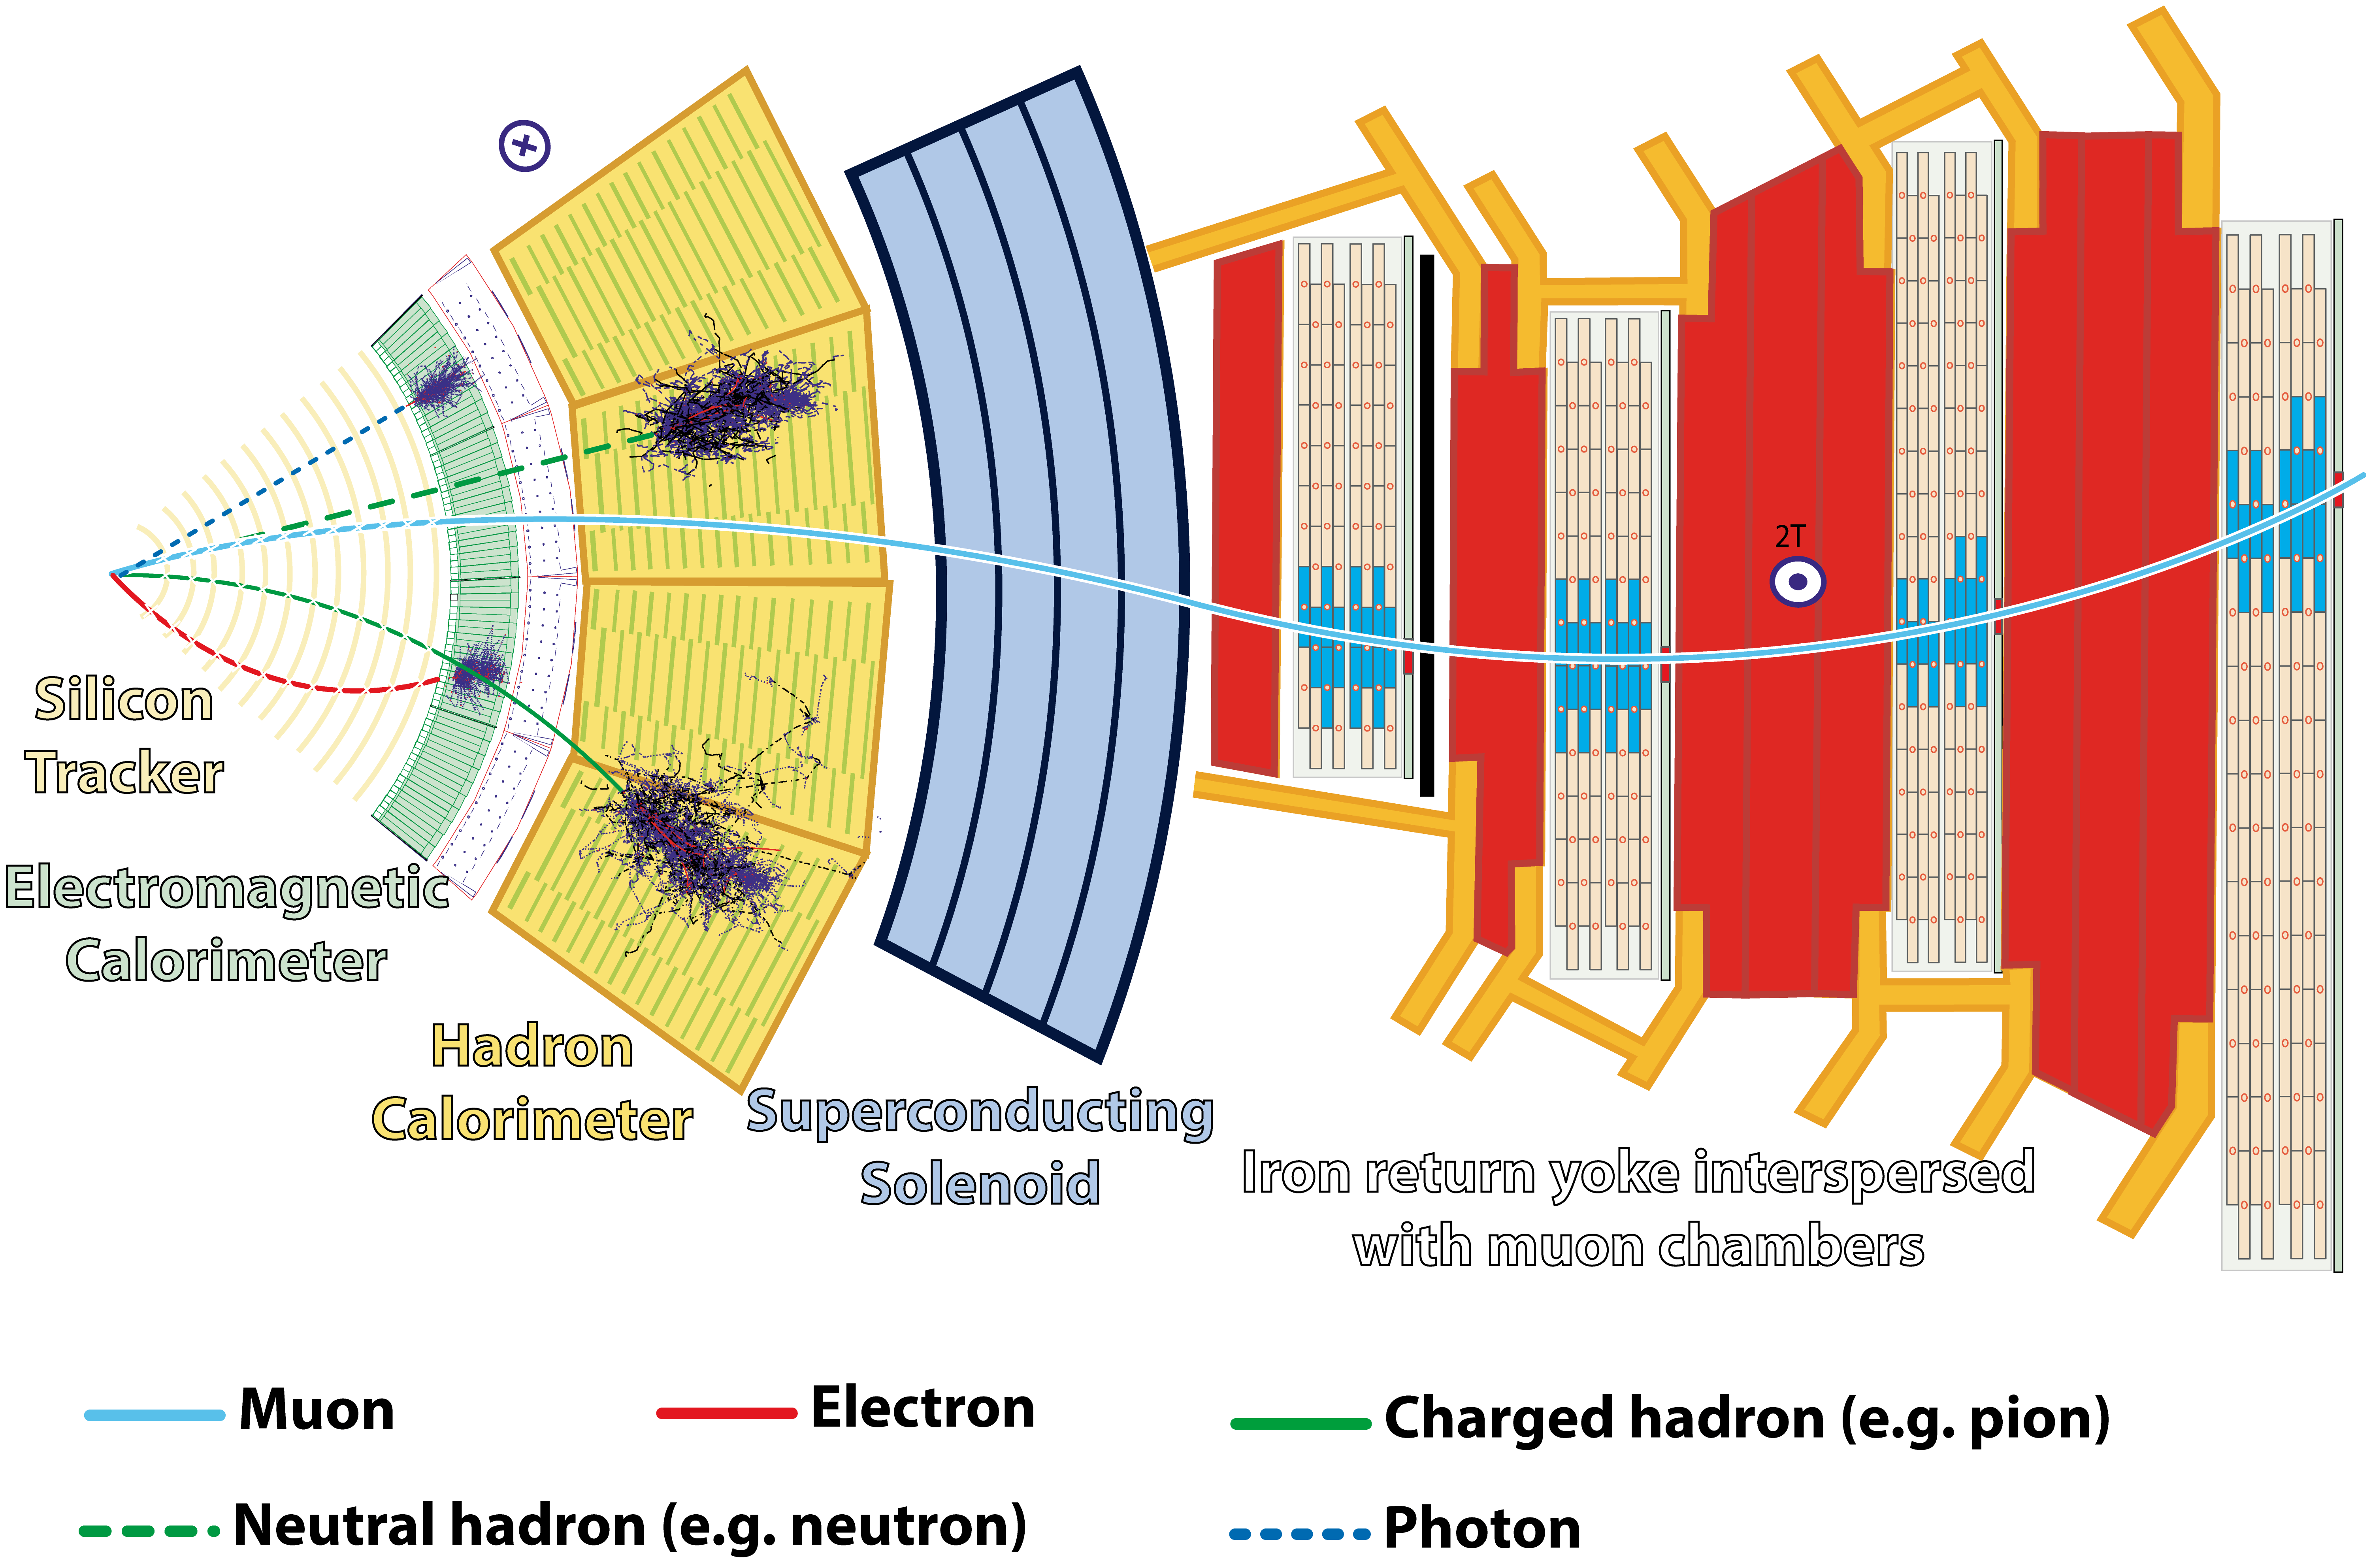
\includegraphics[width=0.8\textwidth]{Figures/CMS Slice White Background.png} % Replace with a Tracker diagram
    \caption{Cross-sectional schematic of the CMS detector}
    \label{fig:cms_tracker}
\end{figure}

\section{Silicon Tracker}

The tracker system in the CMS detector is designed to reconstruct the trajectories of charged particles produced in high-energy collisions with unparalleled precision. This subsystem plays a vital role in measuring the momentum of particles, identifying particle types, and reconstructing primary and secondary vertices.

\subsection{Silicon Pixel Detector}
The innermost layer of the tracker is the silicon pixel detector, which provides high-resolution tracking near the interaction point. It consists of three barrel layers and two endcap disks on either side, covering a pseudorapidity range of $|\eta| < 2.5$ \cite{tracker_tdr}. The pixel detector is constructed using silicon sensors segmented into millions of tiny pixels, each measuring $100\times150~\mu m^2$.

The pixel detector is designed to withstand intense radiation levels and high particle flux near the beamline. Its fine granularity ensures excellent spatial resolution, which is critical for identifying displaced vertices from the decays of short-lived particles such as $B$-mesons and $	au$ leptons ~\cite{pixels}.

\subsection{Silicon Strip Tracker}
Surrounding the pixel detector is the silicon strip tracker, which extends the tracking coverage to larger radii and provides additional layers for trajectory reconstruction. The strip tracker is divided into the Tracker Inner Barrel (TIB), Tracker Outer Barrel (TOB), Tracker Endcaps (TEC), and Tracker Inner Disks (TID). These components collectively cover a radial distance of 20 to 110 cm from the beamline \cite{tracker_tdr}.

The silicon strips are oriented in parallel arrays, with each strip measuring several centimeters in length and a few hundred microns in width. By combining signals from multiple layers, the strip tracker achieves precise momentum measurements and improves the robustness of the trajectory reconstruction. \cite{strips}

\subsection{Material Choices and Performance}
The tracker is constructed entirely from silicon sensors, chosen for their excellent resolution and radiation hardness. Key considerations in the design include:
\begin{itemize}
    \item \textbf{Lightweight support structures:} Minimize material interactions that can scatter particles and degrade tracking performance.
    \item \textbf{Radiation-tolerant electronics:} Ensure reliable operation in the high-radiation environment of the LHC.
    \item \textbf{High granularity:} Allows for precise reconstruction of particle trajectories even in the presence of multiple simultaneous collisions (pile-up).
\end{itemize}

The tracker achieves a transverse momentum resolution of approximately $\Delta p_T / p_T = 1\%$ for particles with $p_T$ around $100~\mathrm{GeV/c}$. This precision enables detailed studies of particle properties, including invariant mass reconstruction and decay vertex identification \cite{tracker_tdr}.

% \begin{figure}[ht]
%     \centering
%     %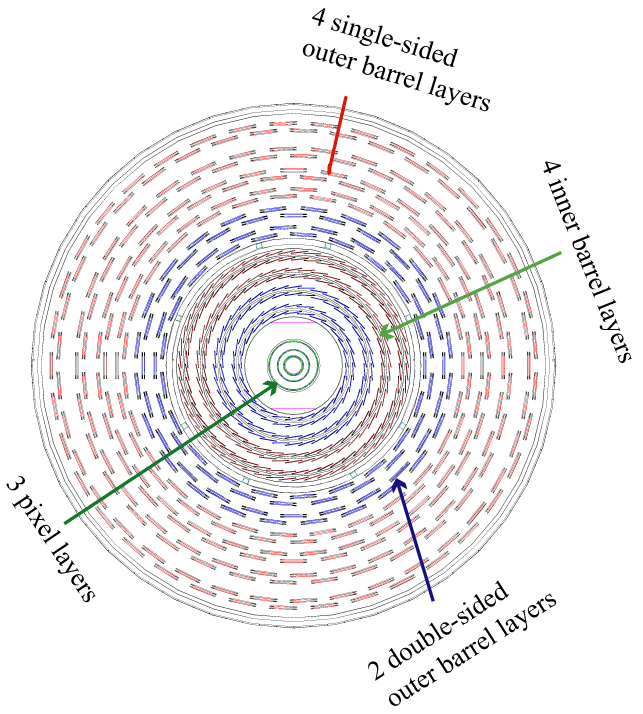
\includegraphics[width=0.8\textwidth]{Figures/Barrel.png} % Replace with a Tracker diagram
%     \caption{Cross-sectional schematic of the CMS tracker, showing the pixel and strip components.}
%     \label{fig:cms_tracker}
% \end{figure}

% \begin{figure}[ht]
%     \centering
%     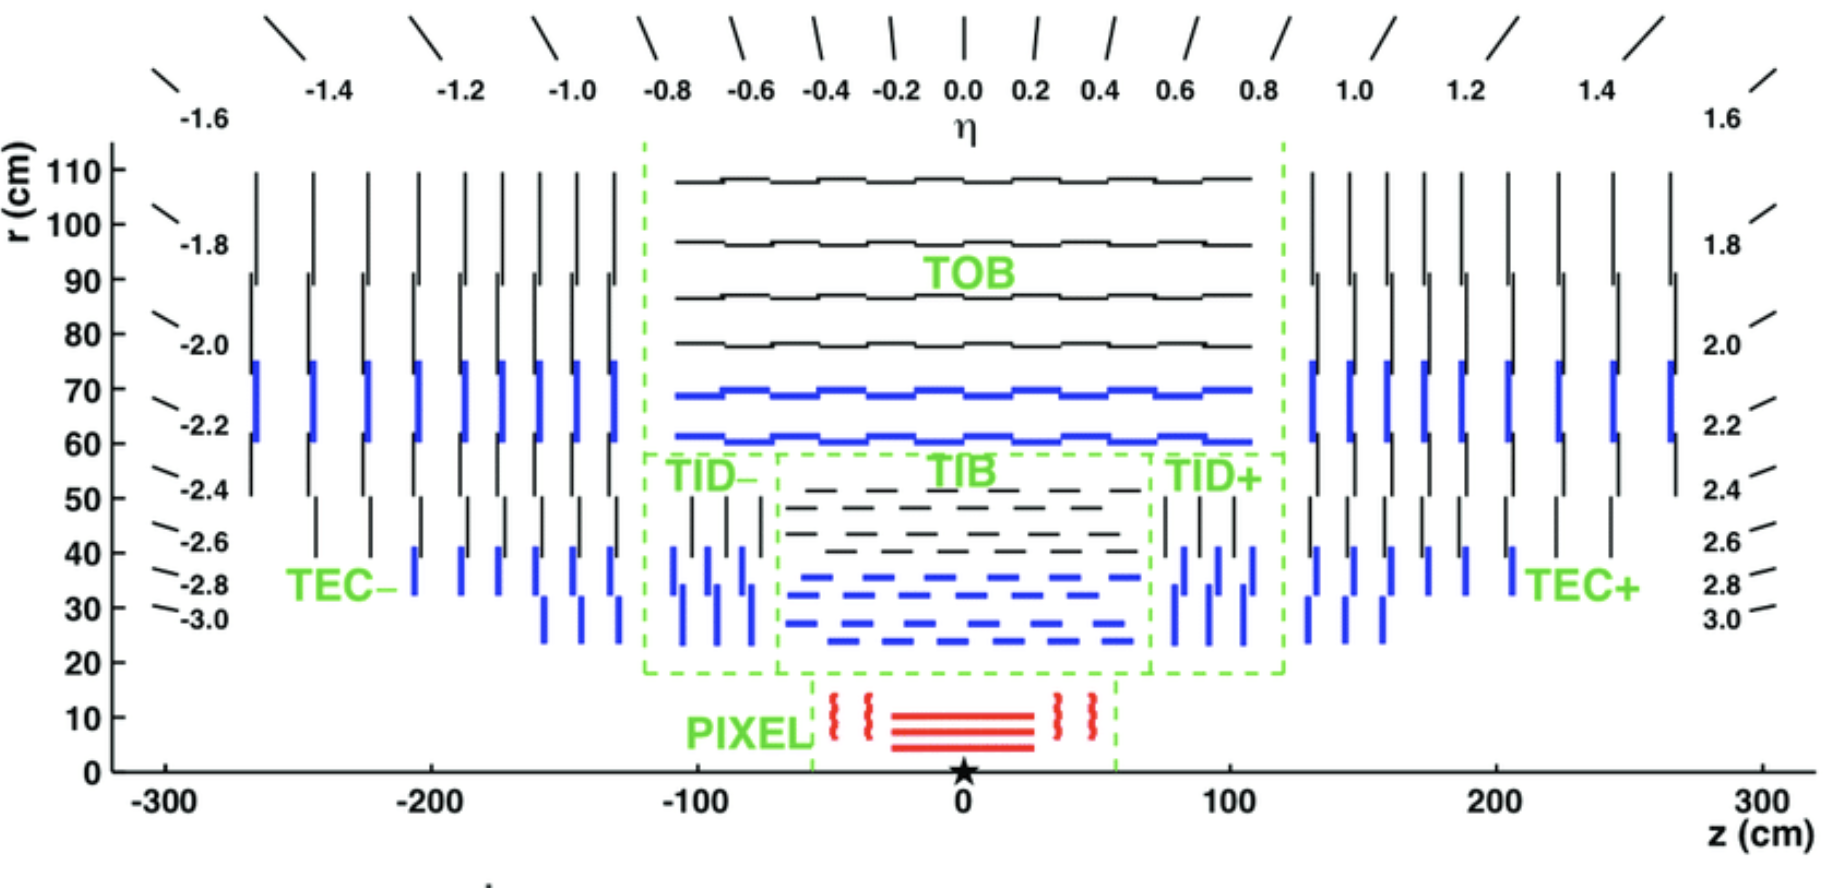
\includegraphics[width=0.8\textwidth]{Figures/tracker_cross.png} % Replace with a Tracker diagram
%     \caption{Cross-sectional schematic of the CMS tracker, showing the pixel and strip components.}
%     \label{fig:cms_tracker}
% \end{figure}

The tracker is designed to withstand high radiation levels and provides a momentum resolution of $\Delta p_T / p_T \approx 1\%$ for particles with $p_T \sim 100~\mathrm{GeV/c}$. The low-mass design minimizes material interactions, reducing the impact on photon and electron measurements. Cooling systems maintain stable operation despite the intense radiation environment.

\section{Electromagnetic Calorimeter (ECAL)}
% The ECAL measures the energy of photons and electrons with high precision. It consists of lead tungstate (PbWO$_4$) crystals, optimized for:
% \begin{itemize}
%     \item Fast response time ($<25~\mathrm{ns}$).
%     \item Radiation hardness.
%     \item Fine granularity for excellent position resolution.
% \end{itemize}



% \subsection{Barrel and Endcap Structure}
% The ECAL is divided into the barrel (EB) and two endcaps (EE), covering $|\eta| < 3.0$. The barrel consists of 36 supermodules, each containing thousands of crystals aligned quasi-projectively to the interaction point. The endcaps extend the coverage to higher pseudorapidities, crucial for forward physics measurements.

% \subsection{Preshower Detector}
% Due to the structure of parallel alignment of crystals in the endcaps, the ECAL has a lower granularity in the endcaps than in the barrel. In order to improve the sensitivity of track of the photons. The endcaps include a preshower detector, comprising two layers of silicon strip sensors placed behind lead converters. This subsystem enhances the discrimination between photons and neutral pions by measuring the photon conversion probability.


% \subsection{Performance}
% Energy resolution is parameterized as:\cite{cms_tdr_ecal}
% \[
% \frac{\sigma_E}{E} = \frac{S}{\sqrt{E}} \oplus \frac{N}{E} \oplus C,
% \]
% where $S$, $N$, and $C$ are the stochastic, noise, and constant terms, respectively. The ECAL achieves an exceptional energy resolution of approximately 1\% for electrons and photons at $E = 100~\mathrm{GeV}$.

The Electromagnetic Calorimeter (ECAL) in the CMS detector is a crucial subsystem designed to measure the energy of electrons and photons with high precision. The ECAL achieves this by utilizing scintillating lead tungstate (PbWO$_4$) crystals as the active medium, coupled with photodetectors to convert scintillation light into electrical signals. Its design, divided into the Barrel (EB), Endcap (EE), and Preshower Detector (ES), ensures optimal performance across a wide range of pseudorapidity. In this research, because our dataset is mainly focused on photons and electrons, the ECAL is actually the region we mainly focus on. In later Chapter, the detector we called is actually reference to the ECAL.

\subsection{The ECAL Barrel (EB)}
The ECAL Barrel covers the central pseudorapidity region, $|\eta| < 1.479$, and consists of approximately 61,200 PbWO$_4$ crystals. These crystals are characterized by their high density, fast scintillation time, and radiation hardness \cite{ecal_tdr}. Lead tungstate is chosen due to its high density and short radiation length, which allows electromagnetic showers to develop within a compact volume. This compactness ensures that the ECAL can achieve high resolution while fitting within the spatial constraints of the CMS detector.

Each crystal is aligned quasi-projectively towards the interaction point, ensuring minimal gaps in coverage and precise angular resolution. The scintillation light produced in the crystals is detected by avalanche photodiodes (APDs) for the barrel region, which offer excellent sensitivity and radiation resistance \cite{ecal_tdr}.

\subsection{The ECAL Endcap (EE)}
The ECAL Endcap extends the coverage of the ECAL to higher pseudorapidities, from $|\eta| = 1.479$ to $|\eta| = 3.0$. The endcap region is composed of roughly 14,600 PbWO$_4$ crystals, arranged in a geometry optimized for forward physics studies \cite{ecal_tdr}. Due to the higher radiation levels and particle flux in this region, the photodetectors used are vacuum phototriodes (VPTs), which are more robust against radiation damage compared to APDs.

The higher radiation environment in the endcap region also necessitates additional cooling and monitoring systems to maintain the performance of the crystals and photodetectors. The EE plays a critical role in measuring photons and electrons produced at small angles relative to the beamline, ensuring comprehensive detector coverage \cite{ecal_tdr}.

\subsection{The Preshower Detector}
The preshower detector is located in front of the ECAL Endcaps and is designed to enhance the discrimination between photons and neutral pions ($\pi^0$). It consists of two layers of lead absorbers, interleaved with silicon strip sensors \cite{ecal_tdr_preshower}. The lead layers initiate electromagnetic showers, while the silicon sensors measure the spatial distribution of the resulting particles.

This design allows the preshower detector to effectively distinguish between single photons and $\pi^0$ decays, which produce two closely spaced photons. This capability is crucial for improving the ECAL's performance in identifying isolated photons in a high-particle-density environment \cite{ecal_tdr_preshower}.

\begin{figure}[ht]
    \centering
    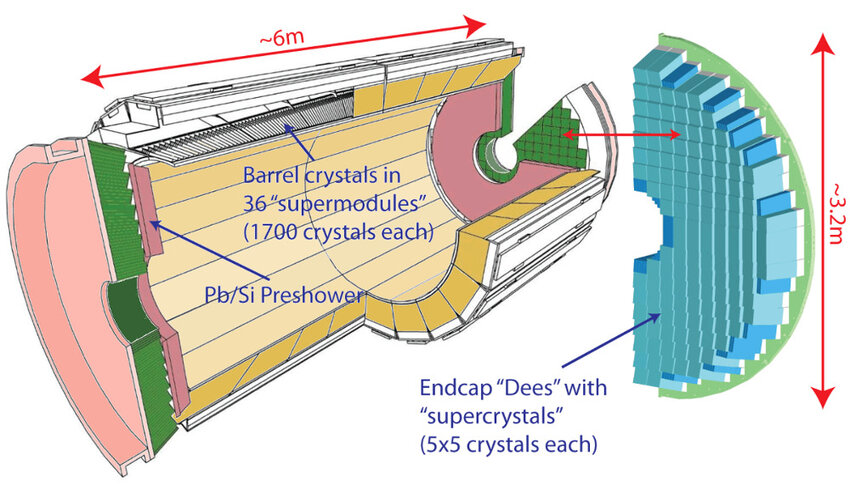
\includegraphics[width=0.8\textwidth]{Figures/ECAL Schematic Overview.png} % Replace with an ECAL diagram
    \caption{Structure of the ECAL showing barrel and endcap regions.} ~\cite{ECAL}
    \label{fig:ecal}
\end{figure}

\subsection{Material Choices and Performance}
The choice of PbWO$_4$ as the active material for the ECAL is driven by its unique properties:
\begin{itemize}
    \item \textbf{High density and short radiation length:} These properties allow electromagnetic showers to be contained within a compact volume, ensuring precise energy measurements.
    \item \textbf{Fast scintillation time:} PbWO$_4$ crystals have a decay time of approximately 25 ns, matching the LHC's bunch crossing interval \cite{ecal_tdr}.
    \item \textbf{Radiation hardness:} PbWO$_4$ is resistant to radiation damage, which is critical for maintaining detector performance over extended periods of operation.
\end{itemize}

The ECAL achieves an excellent energy resolution, parameterized as:

\[
\frac{\sigma_E}{E} = \frac{S}{\sqrt{E}} \oplus \frac{N}{E} \oplus C,
\]

where $S$ is the stochastic term, $N$ represents the noise, and $C$ is the constant term \cite{ecal_tdr}. This resolution allows the ECAL to distinguish between different particle species and measure their energies with high precision, making it an indispensable tool for studies of Higgs boson decays, rare processes, and new physics searches.

\section{Hadronic Calorimeter (HCAL)}
The HCAL measures hadronic energy, complementing the ECAL in reconstructing jets and missing transverse energy. It employs a sampling design with brass absorbers and plastic scintillators.

The Hadronic Calorimeter (HCAL) in the CMS detector is an essential component designed to measure the energy of hadrons produced in high-energy collisions. The HCAL achieves this through a carefully engineered combination of absorber and active materials, divided into distinct regions optimized for different pseudorapidity ranges. These regions include the HCAL Barrel (HB), HCAL Endcap (HE), HCAL Forward (HF), and HCAL Outer (HO). The selection of materials and their specific configurations in each section is driven by the requirements of energy containment, radiation hardness, and detector efficiency.

\subsection{The HCAL Barrel (HB)}
The HCAL Barrel is the central component of the HCAL, covering the region close to the interaction point with a pseudorapidity range of $|\eta| < 1.3$. The HB is constructed using brass as the absorber material and plastic scintillators as the active medium. Brass is chosen due to its high density and structural stability, which allow it to efficiently stop high-energy hadrons and initiate hadronic showers.\cite{hcal_tdr} The dense nature of brass ensures that the hadronic showers are contained within a compact volume, which is critical for the limited space available in the detector.

The active medium in the HB consists of plastic scintillator tiles, which emit light when traversed by charged particles generated in the hadronic showers. This scintillation light is collected by photodetectors, such as silicon photomultipliers, and converted into an electrical signal proportional to the energy deposited in the calorimeter. The use of plastic scintillators ensures a fast response time, high light yield, and excellent linearity, all of which contribute to the precision of energy measurements.

\subsection{The HCAL Endcap (HE)}
The HCAL Endcap extends the coverage of the HCAL to higher pseudorapidities, from $|\eta| = 1.3$ to $|\eta| = 3.0$. Similar to the HB, the HE uses brass as the absorber material and plastic scintillators as the active medium. However, the endcap is designed to handle particles with higher momenta, which require increased thickness of the absorber layers to fully contain the hadronic showers.

The higher density and thickness of the brass absorbers in the HE ensure that the energy of the hadronic showers is completely absorbed, even for particles at extreme angles. The endcap region is critical for capturing the energy of forward jets and particles produced at small angles relative to the beamline, ensuring no significant gaps in the detector's acceptance.\cite{hcal_tdr}

\subsection{The HCAL Forward (HF)}
The HCAL Forward is specifically designed to handle the extreme forward region, covering $3.0 < |\eta| < 5.0$. This region experiences the highest particle flux and radiation levels, necessitating the use of radiation-hard materials such as steel for the absorbers and quartz fibers for the active medium. Steel is chosen for its durability and ability to withstand the intense radiation environment in the forward region. It also provides the density required to stop high-energy hadrons effectively.

The active medium in the HF consists of quartz fibers, which generate Cherenkov light when traversed by relativistic charged particles produced in the hadronic showers. Cherenkov light is collected by specialized photodetectors, providing a robust signal in an environment where plastic scintillators would suffer significant degradation. This combination of materials ensures that the HF maintains its performance over long periods of operation, even in the harshest conditions.

The HF plays a crucial role in studying forward physics phenomena, including parton distribution functions and diffractive events. Its design also contributes to the accurate measurement of missing transverse energy ($E_T^{\text{miss}}$) by reducing the likelihood of undetected particles escaping.\cite{hcal_tdr_forward}

\subsection{The HCAL Outer (HO)}
The HCAL Outer is located outside the superconducting solenoid and complements the energy measurements of the HB. The HO uses the steel return yoke of the solenoid as its absorber, with additional layers of plastic scintillators serving as the active medium. The primary purpose of the HO is to act as a "tail catcher," capturing energy from high-energy particles that pass through the HB and the solenoid without being fully absorbed.

Using the steel return yoke as an integral part of the calorimeter minimizes the overall size and weight of the detector while maintaining its energy containment capabilities. The additional scintillator layers ensure that any residual energy from penetrating particles is measured, providing a complete picture of the event's energy balance. \cite{hcal_tdr_outer}

\subsection{Material Choices and Their Impact}
The material choices for the HCAL are driven by the need to balance density, radiation hardness, and signal quality. Dense materials such as brass and steel are used to contain hadronic showers within a compact volume, minimizing leakage and ensuring precise energy measurements. Plastic scintillators are employed in regions with lower radiation exposure due to their high light yield and fast response time. In contrast, quartz fibers are used in the forward region, where their radiation tolerance and ability to generate Cherenkov light make them the ideal choice.

This careful selection of materials and their strategic placement within the HCAL ensures that the detector meets the stringent requirements for hadronic energy measurement. By providing accurate jet energy reconstruction and missing transverse energy measurements, the HCAL plays a vital role in the CMS detector's ability to explore physics at the energy frontier. \cite{hcal_cms_detector}

\begin{figure}[ht]
    \centering
    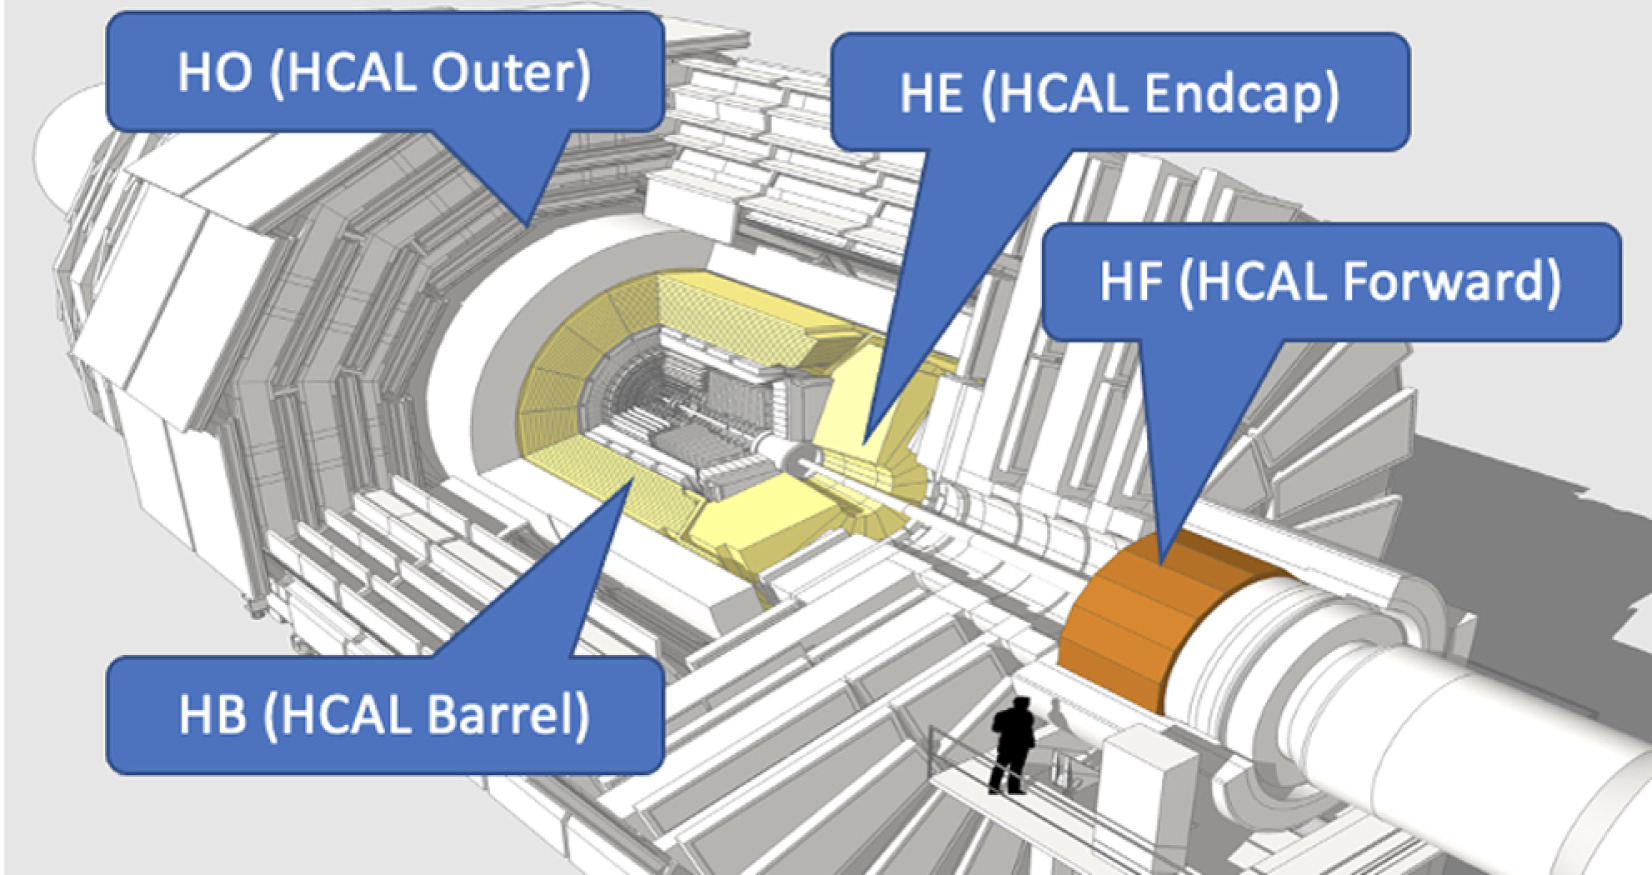
\includegraphics[width=0.8\textwidth]{Figures/HCAL.jpg} % Replace with an HCAL diagram
    \caption{Schematic of the HCAL with barrel, endcap, and forward sections.}
    \label{fig:hcal}
\end{figure}

\subsection{Performance}
The HCAL provides energy resolution of:\cite{cms_tdr_hcal}
\[
\frac{\sigma_E}{E} = \frac{S}{\sqrt{E}} \oplus C.
\]
The combination of ECAL and HCAL ensures accurate jet energy reconstruction and $E_T^{\text{miss}}$ measurements, critical for new physics searches.

\section{Muon Detector}
The muon detector in the CMS experiment is a crucial subsystem designed to identify and measure the momentum of muons, which are often key signatures in high-energy collisions. The muon system provides the outermost layer of the CMS detector, ensuring precise muon tracking and efficient triggering across a wide range of pseudorapidity.

\subsection{Muon Chambers: Drift Tubes (DT)}
Drift tubes are the primary technology used in the barrel region of the CMS detector, covering $|\eta| < 1.2$. They consist of gas-filled chambers with wires running along their length. When a muon passes through the chamber, it ionizes the gas, and the resulting electrons drift toward the central wire under the influence of an electric field \cite{muon_tdr}.

The time taken by the electrons to reach the wire allows for precise measurements of the muon's position. The DTs are arranged in layers, providing redundancy and improving spatial resolution. The use of drift tubes in the barrel region ensures robust performance in areas with lower radiation exposure and relatively uniform magnetic fields.

\subsection{Muon Chambers: Cathode Strip Chambers (CSC)}
Cathode strip chambers are employed in the endcap regions, where the pseudorapidity ranges from $1.2 < |\eta| < 2.4$. The CSCs are designed to operate in areas with higher radiation levels and non-uniform magnetic fields. They consist of multi-layered gas chambers with cathode strips and anode wires arranged perpendicularly \cite{muon_tdr}.

When a muon traverses a CSC, it ionizes the gas, and the resulting charge is collected on the strips and wires. The perpendicular arrangement allows for precise two-dimensional position measurements. This design ensures high efficiency and excellent spatial resolution in the endcap regions, where particle flux and radiation are more intense \cite{muon_tdr}.

\subsection{Resistive Plate Chambers (RPC)}
Resistive plate chambers are used in both the barrel and endcap regions, providing fast timing information and additional redundancy for triggering. RPCs consist of parallel resistive plates separated by a thin gas layer. When a muon passes through the gas, it creates an avalanche of electrons, resulting in a detectable signal \cite{muon_tdr}.

The fast response time of RPCs makes them ideal for the Level-1 trigger system, which is responsible for selecting events of interest in real time. Their simple design and robust performance contribute significantly to the overall efficiency of the muon detector.

\subsection{Material Choices and Performance}
The materials and technologies used in the muon detector are carefully chosen to meet the demands of high-energy particle physics experiments:
\begin{itemize}
    \item \textbf{Gas-filled chambers:} Used in DTs and CSCs for their ability to provide precise spatial measurements and operate in high-radiation environments.
    \item \textbf{Resistive materials:} Employed in RPCs to ensure fast timing and robust performance under high particle flux.
    \item \textbf{Redundant layering:} Multiple layers of chambers improve tracking resolution and ensure reliability in detecting muons.
\end{itemize}

The muon system achieves a momentum resolution of $\Delta p / p \sim 10\%$ at $1~\mathrm{TeV/c}$, enabling precise measurements of high-momentum muons \cite{muon_tdr}. This capability is critical for identifying rare processes, such as those involving heavy bosons or new particles.

\begin{figure}[ht]
    \centering
    %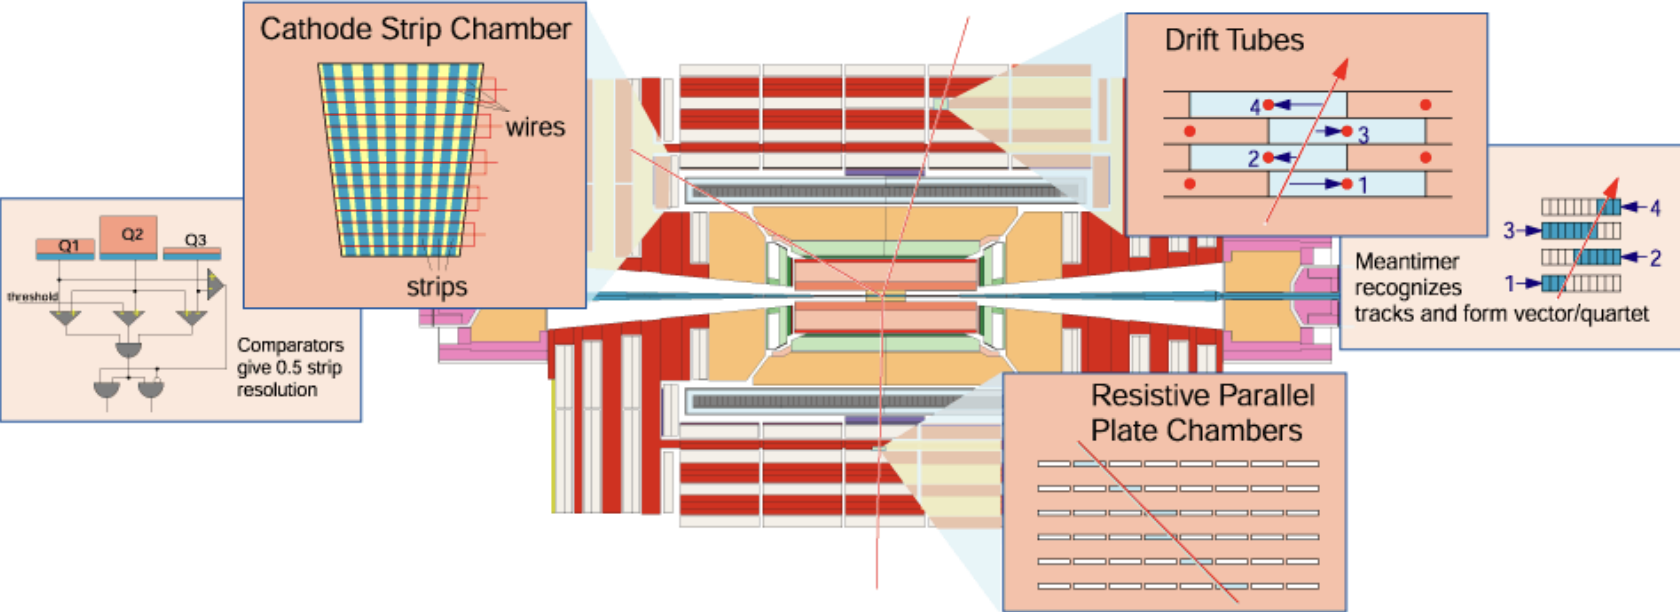
\includegraphics[width=0.8\textwidth]{muon_detector.png} % Replace with a Muon Detector diagram
    \caption{CMS Muon System layout, showing DTs, CSCs, and RPCs.}
    \label{fig:muon_detector}
\end{figure}

The muon system achieves momentum resolution of $\Delta p / p \sim 10\%$ at $1~\mathrm{TeV/c}$, contributing significantly to global track reconstruction.\cite{cms_tdr_muon}

\subsection{Trigger and Reconstruction}
The CMS trigger system is essential for managing the vast amount of data generated by the detector, selecting only the most relevant events for further analysis. The trigger operates in two levels: the Level-1 Trigger and the High-Level Trigger (HLT).

\subsection{Level-1 Trigger}
The Level-1 Trigger is a hardware-based system designed to process data in real time and reduce the event rate from 40 MHz to approximately 100 kHz \cite{trigger_tdr}. It uses custom electronics located close to the detector to analyze data from the calorimeters and muon chambers. This system identifies candidate particles such as muons, electrons, and jets, and makes decisions within microseconds.

The Level-1 Trigger ensures that only events with significant physics potential, such as those involving high-energy muons or missing transverse energy, are passed on to the next stage \cite{trigger_tdr}.

\subsection{High-Level Trigger (HLT)}
The High-Level Trigger is a software-based system that further reduces the event rate from 100 kHz to approximately 1 kHz, suitable for storage and offline analysis \cite{trigger_tdr}. The HLT uses a computing farm to reconstruct full events in real time, applying more sophisticated algorithms to refine the selection criteria.

This stage enables detailed analysis of particle trajectories and energy deposits, ensuring that only the most promising events are retained for later study. The combination of the Level-1 Trigger and HLT allows CMS to efficiently manage the enormous data flow while preserving the ability to capture rare and significant physics phenomena.


\section{Conclusion}
The CMS detector integrates advanced subsystems, including the tracker, calorimeters, and muon chambers, to provide comprehensive coverage and high precision. These capabilities enable CMS to explore the rich physics opportunities at the LHC.
